%20 min preso!
\documentclass[xcolor=table,english]{beamer}
\usepackage{beamerthemesplit}
\usepackage{wrapfig}
\usetheme{SPbGU}
\usepackage{pdfpages}
\usepackage{amsmath}
\usepackage{mathtools}
\usepackage{cmap}
\usepackage{subcaption}
\usepackage[utf8]{inputenc}
\usepackage[T1, T2A]{fontenc}
\usepackage[]{babel}
\usepackage{indentfirst}
\usepackage{amsmath}
\usepackage{tikz}
\usepackage{multirow}
\usepackage[noend]{algpseudocode}
\usepackage{algorithm}
\usepackage{algorithmicx}
\usepackage{fancyvrb}
\usetikzlibrary{calc}
\usetikzlibrary{shapes,arrows}
\usetikzlibrary{arrows,automata}
\usetikzlibrary{positioning}
\usetikzlibrary{fit}

\usepackage{kbordermatrix} % include package @ document preamble
\renewcommand{\kbldelim}{(} % change default array delimiters to parentheses
\renewcommand{\kbrdelim}{)}

\newcommand\mca{\multicolumn{1}{c}{\cellcolor{red}\textbf{\{a\}}}}
\newcommand\mcb{\multicolumn{1}{c}{\cellcolor{red}\textbf{\{b\}}}}

\usepackage{tabularx}
\newcolumntype{Y}{>{\raggedleft\arraybackslash}X}

\renewcommand{\thealgorithm}{}

\newtheorem{mytheorem}{Theorem}
\renewcommand{\thealgorithm}{}

\newcommand{\tikzmark}[1]{\tikz[overlay,remember picture] \node (#1) {};}
\def\Put(#1,#2)#3{\leavevmode\makebox(0,0){\put(#1,#2){#3}}}

\newcommand{\ltz}{$< 1$}


\tikzset{
    state/.style={
           rectangle,
           rounded corners,
           draw=black, very thick,
           minimum height=2em,
           inner sep=2pt,
           text centered,
           },
}

\beamertemplatenavigationsymbolsempty

\title[Flow2Vec]{Flow2Vec: Value-Flow-Based Precise Code Embedding}
\subtitle[YaccConstructor]{Applications of CFPQ analysis}
% То, что в квадратных скобках, отображается в левом нижнем углу.
\institute[СПбГУ]{
JetBrains Research, Лаборатория языковых инструментов  \\
Санкт-Петербургский Государственный университет
}

% То, что в квадратных скобках, отображается в левом нижнем углу (прикольно).
\author[Егор Орачев]{\textbf{Егор Орачев}}
\date{22 марта 2021}


\begin{document}
{
\begin{frame}[fragile]
  \begin{table}
  \centering
  \begin{tabularx}{\linewidth}{YcX}
    
\includegraphics[height=1.5cm]{pictures/jetbrainsResearch.pdf} \hfill
    & \begin{minipage}[t]{0.3\textwidth}\center \vspace{-1cm}  Семинар
      \end{minipage}
    & \hfill 
\includegraphics[height=1.5cm]{pictures/SPbGU_Logo.png}
  \end{tabularx}
  \end{table}
  \titlepage
\end{frame}
}

\begin{frame}[fragile] \frametitle{Предметная область}
    \begin{minipage}[m]{0.45\linewidth}
        \begin{figure}
            \centering
            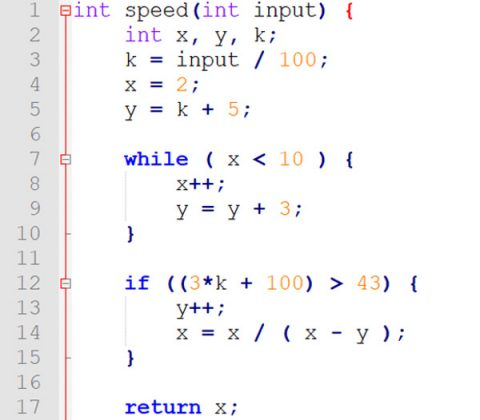
\includegraphics[width=0.8\textwidth]{figures/static_code_analysis.jpg}
            \caption{Code fragment}
            \label{fig:code_fragment}
        \end{figure}
    \end{minipage}\hfill
    \begin{minipage}[m]{0.55\linewidth}
        \textbf{Статический анализ кода}
        \begin{itemize}
            \item Interprocedural data flow analysis
            \item Program slicing
            \item Pointer  analysis
            \item Shape analysis
            \item Code classification
            \item Code summarization
        \end{itemize}
    \end{minipage}
\end{frame}

\begin{frame}[fragile] \frametitle{Представление программы}
    \begin{itemize}
        \item Проблема: эффективность анализа зависит от того, насколько "хорошим" является используемое представление программы
        \item Варианты: 
        {
            \begin{itemize}
                \item Абстрактное синтаксическое дерево
                \item Представление в промежуточном языке
                \item Граф потока данных
                \item Граф потока управления
                \item Граф вызовов
                \item Представление программы в виде embedding'а
            \end{itemize}
        }
    \end{itemize}
\end{frame}

\begin{frame}[fragile] \frametitle{Структура презентации}
    \begin{itemize}
        \item Code2vec: метод и его описание
        \item Построение embedding'а для ориентированного графа
        \item Запросы с контекстно-свободными (КС) ограничениями
        \item Flow2vec: метод и его описание
        \item Flow2vec: практическое применение
        \item Наши исследования в области вычисления КС запросов
        \item Дальнейшее направление исследований  
    \end{itemize}
\end{frame}

\begin{frame}[fragile] \frametitle{Graph Embedding}
    \begin{itemize}
        \item Построение представления графа в векторном пространстве выбранной размерности
        {
            \begin{itemize}
                \item Вершины графа --- это вектора
                \item Можно использовать в задачах реконтсрукции графа, рекомендации соседей, предстказания связей и т.д.
            \end{itemize} 
        }
        \item Проблемы:
        {
            \begin{itemize}
                \item Необходимо сохранить "важные" свойства графа
                \item Реальные графы является ориентированными и обладают ассиметричной транзитивностью
            \end{itemize}
        }
    \end{itemize}
\end{frame}

\begin{frame}[fragile] \frametitle{Graph Embedding: Идея}
    \begin{minipage}[m]{\linewidth}
        \begin{figure}
            \centering
            \begin{subfigure}[b]{0.45\textwidth}
                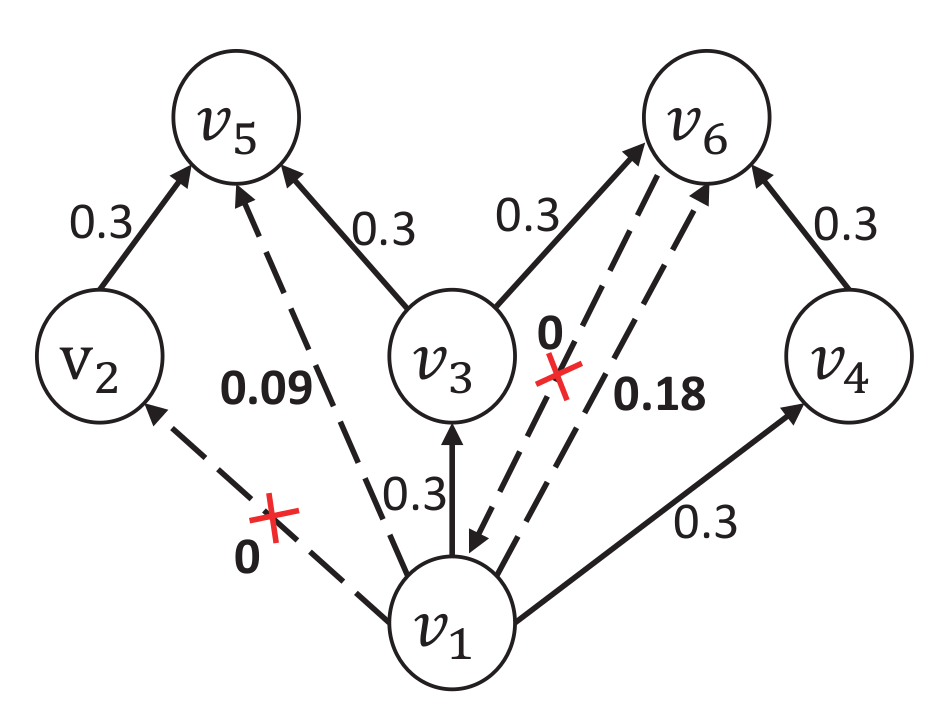
\includegraphics[width=\textwidth]{figures/hope_graph.png}
                \caption{Directed graph}
            \end{subfigure}
            \hfill
            \begin{subfigure}[b]{0.45\textwidth}
                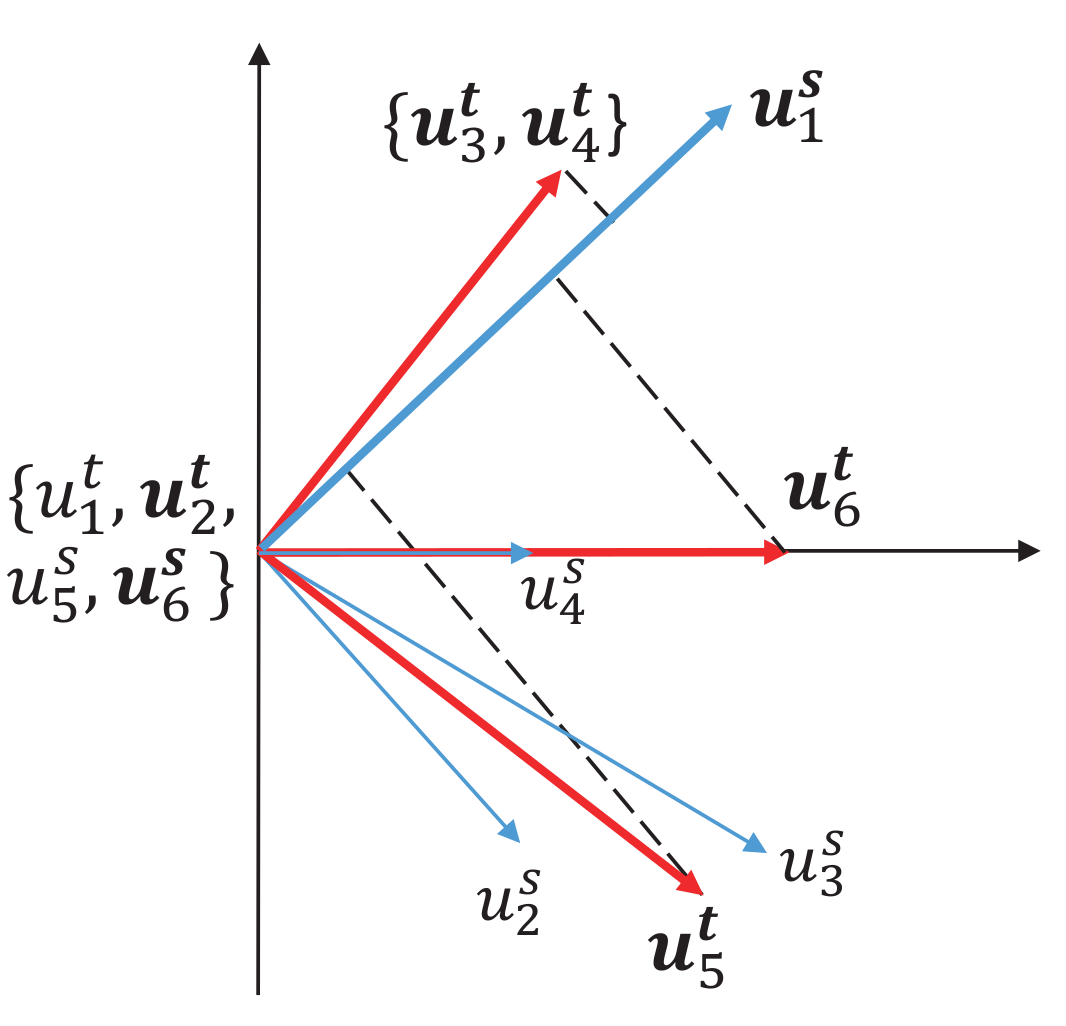
\includegraphics[width=\textwidth]{figures/hope_embedding.png}
                \caption{Graph embedding}
            \end{subfigure}
            \caption{HOPE: Asymmetric Transitivity Preserving Graph Embedding}
        \end{figure}
    \end{minipage}\hfill
\end{frame}

\begin{frame}[fragile] \frametitle{Graph Embedding: Постановка задачи}
    \begin{itemize}
        \item Ориентированный граф $G = \langle V, E \rangle$, $V = \{ v_1, ... , v_N \}$, $|V| = N$, $e_{ij}=(v_1, v_2) \in E$
        \item Матрица смежности графа $A \in \mathbb{R}^{N \times N}$, $a_i$ - i-ая строка матрицы, $A_{ij}$ - элемент матрицы в i-ой строке и j-том столбце
        \item Матрица $S \in \mathbb{R}^{N \times N}$ - матрица близости графа
        \item Embedding матрицы $U = [U^s, U^t]$, $U^s, U^t \in \mathbb{R}^{N \times K}$, $K \in \mathbb{N}$ - размерность emdedding'а, вектора $u^s_i, u^t_i$ соответсвуют вершине графа $v_i$
        \item \textbf{Хотим приблизить матрицу $S$ оптимально в следующем смысле $min \| S - U^s * {U^t}^T \|^2_F$, где $\| \bullet \|_F$ - норма Фробениуса} 
    \end{itemize}
\end{frame}

\begin{frame}[fragile] \frametitle{Graph Embedding: High-order Proximity Matrix}
    \begin{itemize}
        \item Построение матрицы близости $S$, которая сохранит "важные" свойства графа для дальнейшего анализа
        \item Варианты выбора $S$:
        {
            \begin{itemize}
                \item Индекс Катца (англ. Katz index): \\$S^{Katz} = \Sigma_{i=1}^{\infty} \beta^i A^i$, где $\beta \in (0, 1)$ - фактор ослабления
                \item Rooted PageRank
                \item Common Neighbors
                \item Adamic-Adar
            \end{itemize}
        }
        \item Только Katz index и Rooted PageRank сохраняют глобальную ассиметричную транзитивность графа
    \end{itemize}
\end{frame}

\begin{frame}[fragile] \frametitle{Graph Embedding: Approximation of High-Order Proximity}
    \begin{itemize}
        \item $S = S^{Katz} = \Sigma_{i=1}^{\infty} \beta^i A^i$, \\$S^{Katz} = \beta A * S^{Katz} + \beta * A$, $S^{Katz} = (I - \beta A)^{-1} * \beta A$
        \item $S = \Sigma_{i=1}^N \sigma_i v_i^s {v_i^t}^T$ используя SVD разложение, где $\{\sigma_1, ... , \sigma_N\}$ сингулярные значения в порядке убывания
        \item $U^s = [ \sqrt{\sigma_1} * v_1^s, ..., \sqrt{\sigma_K} * v_K^s ]$
        \item $U^t = [ \sqrt{\sigma_1} * v_1^t, ..., \sqrt{\sigma_K} * v_K^t ]$
        \item Ошибка аппроксимации: $\| S - U^s * {U^t}^T \|^2_F = \Sigma_{i=K+1}^N \sigma_i^2$
        \item Относительная ошибка аппроксимации: $\dfrac{\| S - U^s * {U^t}^T \|^2_F}{\| S \|^2_F} = \dfrac{\Sigma_{i=K+1}^N \sigma_i^2}{\Sigma_{i=1}^N \sigma_i^2}$
    \end{itemize}
\end{frame}

\begin{frame}[fragile] \frametitle{Graph Embedding: Итоги}
    \begin{itemize}
        \item Для ориентированного графа $G$ можем построить embedding, который сохраняет ассиметричную транзитивность графа
        \item Для построения требуется матрица близости высокого порядка $S$, которая сохраняет 
        глобальную ассиметричную транзитивность графа
        \item Полученный embedding $U = [U^s, U^t]$ обладает имеет доказанные оценками ошибки приближения. Значение ошибки можно уменьшить, увеличив значение параметра $K$
    \end{itemize}
\end{frame}

\begin{frame}[fragile] \frametitle{Context-free Path Querying}
    \begin{minipage}[m]{0.45\linewidth}
        \begin{figure}
            \centering
            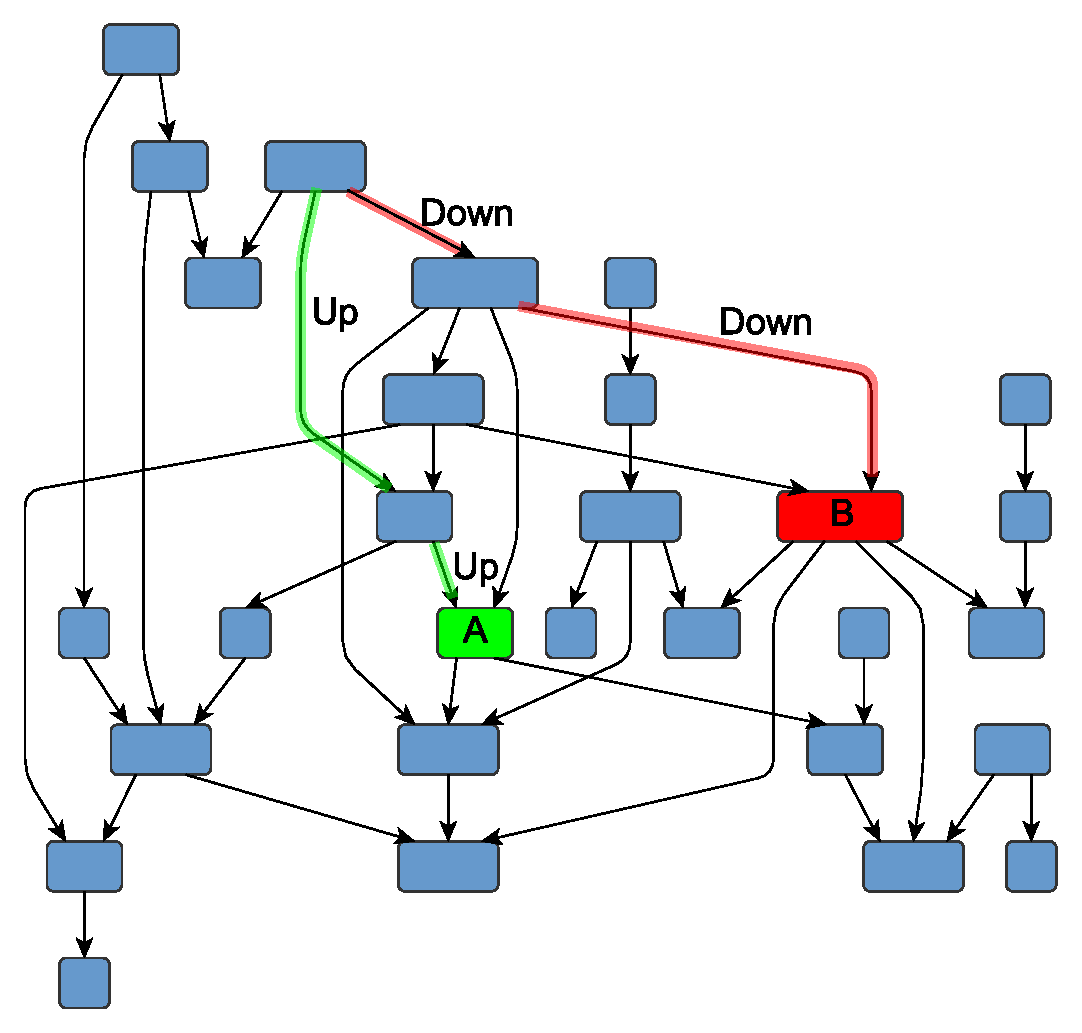
\includegraphics[width=0.8\textwidth]{pictures/hierarchical.pdf}
            \caption{Example of a graph}
        \end{figure}
    \end{minipage}\hfill
    \begin{minipage}[m]{0.55\linewidth}
        \textbf{Навигация в графе:}
        \begin{itemize}
            \item Находятся ли вершины A и B на одном уровне иерархии?
            \item Существует ли путь вида $\textbf{Up}^n \, \textbf{Down}^n$?
            \item Найти все такие пути $\textbf{Up}^n \, \textbf{Down}^n$, которые начинаются в вершине~А
        \end{itemize}
    \end{minipage}
\end{frame}

\begin{frame}[fragile] \frametitle{Context-free Path Querying: Применение}
    \begin{itemize}
        \item Графовые базы данных\footnote{Querying Graph Databases, Pablo Barceló Baeza,  \href{https://doi.org/10.1145/2463664.2465216}{https://doi.org/10.1145/2463664.2465216}}
        \item Анализ RDF данных\footnote{Context-Free Path Queries on RDF Graphs, Xiaowang Zhang, Zhiyong Feng, Xin Wang et al., \href{https://arxiv.org/abs/1506.00743}{https://arxiv.org/abs/1506.00743}}
        \item Биоинформатика\footnote{Quantifying variances in comparative RNA secondary structure prediction, James Anderson, Adám Novák, Zsuzsanna Sükösd et al., \href{https://bmcbioinformatics.biomedcentral.com/articles/10.1186/1471-2105-14-149}{https://bmcbioinformatics.biomedcentral.com/articles/10.1186/1471-2105-14-149}}
        \item Статический анализ кода\footnote{Fast Algorithms for Dyck-CFL-Reachability with Applications to Alias Analysis, Qirun Zhang, Michael R. Lyu, Hao Yuan, Zhendong Su, \href{https://doi.org/10.1145/2499370.2462159}{https://doi.org/10.1145/2499370.2462159}}
    \end{itemize}
\end{frame}

\begin{frame}[fragile] \frametitle{Context-free Path Querying: Терминология}
    \begin{itemize}
        \item Ориентированный граф с меткаи $\mathcal{G} = \langle V, E, L \rangle$
        \item $\omega(\pi) = \omega(v_0 \xrightarrow{l_0} v_1 \xrightarrow{l_1} \cdots \xrightarrow{l_{n-2}} v_{n-1} \xrightarrow{l_{n-1}} v_n) = l_0 l_1 \cdots l_{n-1}$
        \item КС Грамматика $G = \langle \Sigma, N, P, S \rangle$
        \item Язык $L(G) = \{ w~|~S \rightarrow^*_G w \}$
        \item Семантика достижимости: $R = \{ (u, v) ~|~ \exists u \pi v: \omega(\pi) \in L \}$
        \item Семантика всех путей: $\Pi = \{ u \pi v ~|~ \omega(\pi) \in L \}$
    \end{itemize}
\end{frame}

\begin{frame}[fragile] \frametitle{Context-free Path Querying: Пример}
    \begin{minipage}[m]{\linewidth}
        \begin{figure}
           \centering
            \begin{subfigure}[b]{0.4\textwidth}
                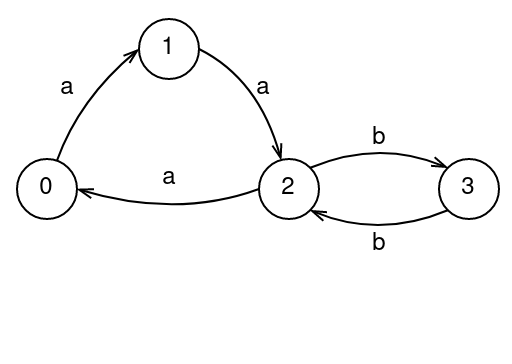
\includegraphics[width=\textwidth]{figures/graph_cfpq_1.png}
                \caption{input graph}
            \end{subfigure}
            \hfill
            \begin{subfigure}[b]{0.4\textwidth}
                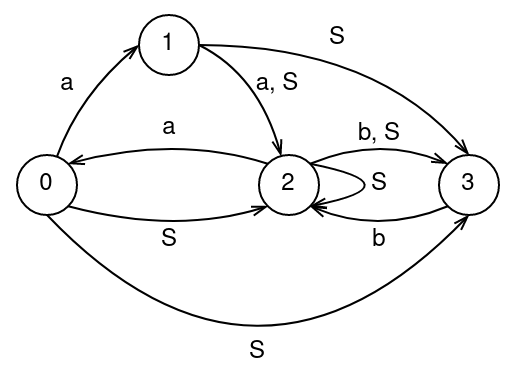
\includegraphics[width=\textwidth]{figures/graph_cfpq_2.png}
                \caption{Result graph}
            \end{subfigure}
            \caption{CFPQ Example}
        \end{figure}
    \end{minipage}\hfill
    \begin{minipage}[m]{\linewidth}
        \begin{itemize}
            \item Грамматика $S \rightarrow aSb~|~ab$
            \item Резульат (Семантика достижимости): ребра с меткой S
            \item Резульат (Семантика всех путей): $\{1 \xrightarrow{a} 3, 0 \xrightarrow{a} 1 \xrightarrow{a} 2 \xrightarrow{b} 3 \xrightarrow{b} 2, 1 \xrightarrow{a} 2 \xrightarrow{a} 0 \xrightarrow{a} 1 \xrightarrow{a} 2 \xrightarrow{b} 3 \xrightarrow{b} 2 \xrightarrow{b} 3 \xrightarrow{b} 2, ...\}$
        \end{itemize}
    \end{minipage}
\end{frame}

\begin{frame}[fragile] \frametitle{Context-free Path Querying: Существующие алгоритмы}
    \begin{itemize}
        \item Алгоритмы, основанные на различных техниках парсинга\\(CYK, LL, LR, etc.)
        \item \textbf{Алгоритмы, основанные на линейной алгебре}
        {
            \begin{itemize}
                \item Матричный алгоритм Рустама Азимова
                \\- семантика: достижимости, одного пути, всех путей
                \\- платформа: CPU, GPU
                \item Алгоритм на основе пересечения графа и рекурсивного автомата через произведения Кронекера
                \\- семантика: достижимости, одного пути, всех путей
                \\- платформа: CPU, GPU
            \end{itemize}
        }
    \end{itemize}
\end{frame}

\begin{frame}[fragile] \frametitle{Context-free Path Querying: Итоги}
    \begin{itemize}
        \item Для анализа графа можем задавать запросы с КС ограничениями
        \item Для каждой конкретной задачи можем выбирать различную семантику запроса
        \item Имеем ээфективные алгоритмы для вычисления запросов на двух основных вычислительных платформах
    \end{itemize}
\end{frame}

\begin{frame}[fragile] \frametitle{Code Embedding: Предыстория}
    \begin{itemize}
        \item Развитие техник embedding'а в области обработки и анализа естественных языков (word2vec, и т.д.)
        \item Развитие техник code embedding'а для построения представления программ (code2vec, и т.д.)
    \end{itemize}
\end{frame}

\begin{frame}[fragile] \frametitle{Code Embedding: Мотивация}
    \begin{itemize}
        \item Развитие техник embedding'а в обрабокте естественных языков
        \item Code embedding'и в качестве представления программ
        \item Методы машинного обучения для анализа программ по новому представлению
    \end{itemize}
\end{frame}

\begin{frame}[fragile] \frametitle{Code Embedding: Проблемы}
    \begin{minipage}[m]{\linewidth}
        \begin{figure}
            \centering
            \begin{subfigure}[b]{0.35\textwidth}
                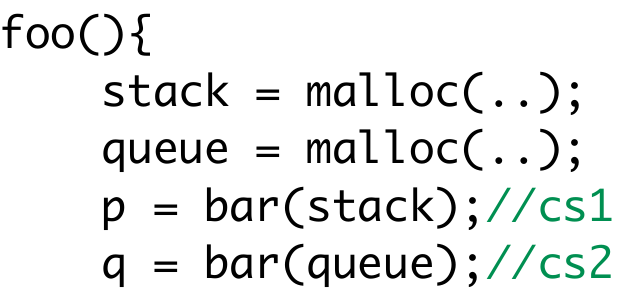
\includegraphics[width=\textwidth]{figures/code_for_ast.png}
                \caption{Foo function}
            \end{subfigure}
            \hfill
            \begin{subfigure}[b]{0.55\textwidth}
                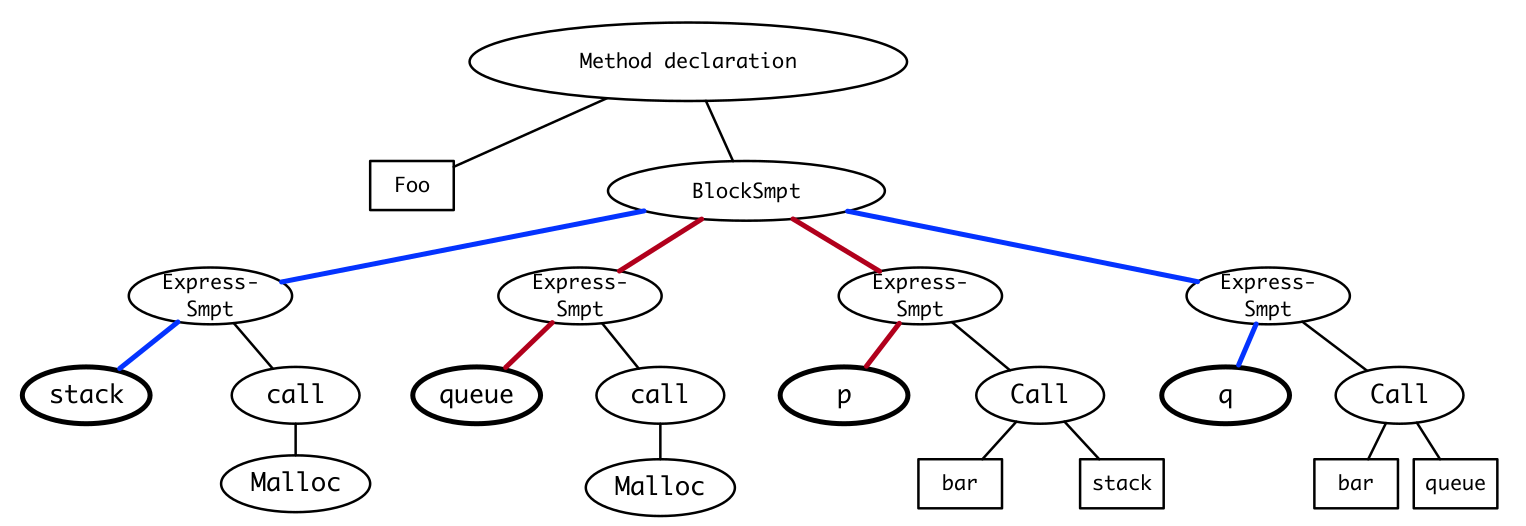
\includegraphics[width=\textwidth]{figures/ast_approach.png}
                \caption{Ast for foo}
            \end{subfigure}
            \caption{Spurious paths example}
        \end{figure}
    \end{minipage}\hfill
    \begin{minipage}[m]{\linewidth}
        \begin{itemize}
        \item Существующие интсрументы
            {
            \begin{itemize}
                \item Code2vec
                \item Code2seq
                \item Word2vec-like ...
            \end{itemize}
            }
            \item Недостатки
            {
            \begin{itemize}
                \item Не учитывают меж-процедурное взаимодействие
                \item Не учитывают псевдонимы (ссылки)
                \item Не учитывают ассиметричную транзитивность программ
            \end{itemize}
            }
        \end{itemize}
    \end{minipage}
\end{frame}

\begin{frame}[fragile] \frametitle{Flow2Vec}
    \begin{itemize}
            \item Новый алгоритм, предложенный в статье \textit{Flow2Vec: Value-Flow-Based Precise Code Embedding}\footnote{Ссылка: \href{https://dl.acm.org/doi/10.1145/3428301}{https://dl.acm.org/doi/10.1145/3428301}} 
            \item Учитывает ранее указанные недостатки
            \item Использует Intermediate Representation (IR), Interprocedural Value-Flow Graph (IVFG) и  CFPQ для построяния value-flow reachability матриц
        \end{itemize}
\end{frame}

\begin{frame}[fragile] \frametitle{Flow2Vec: Алгоритм}
    \begin{minipage}[m]{\linewidth}
        \begin{figure}
            \centering
            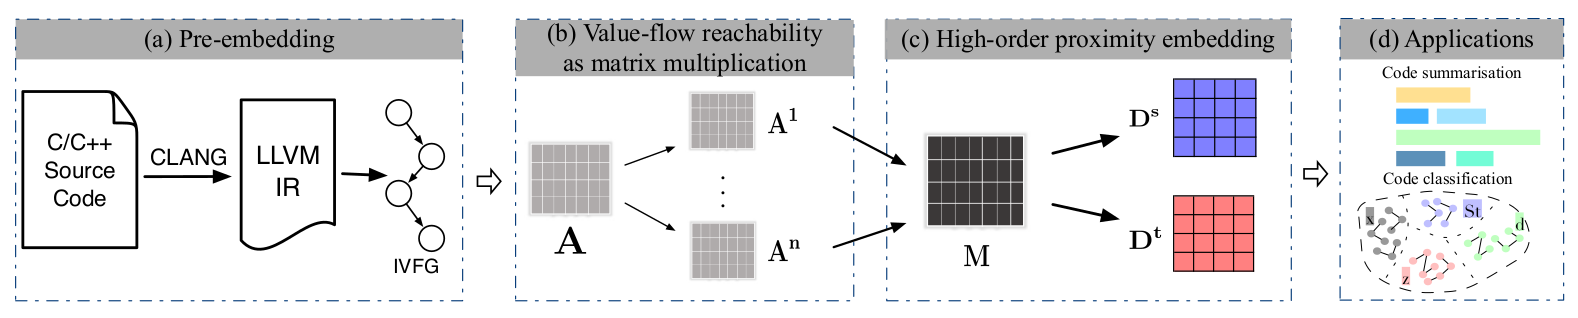
\includegraphics[width=0.8\textwidth]{figures/flow2vec_idea.png}
            \caption{Flow2vec idea}
            \label{fig:flow2vec_idea}
        \end{figure}
    \end{minipage}\hfill
    \begin{minipage}[m]{\linewidth}
        \begin{itemize}
            \item Шаг 1: Построение IR, IVFG, исходных матриц с call/return и value-flow информацией
            \item Шаг 2: Value-flow reachability через CFPQ
            \item Шаг 3: Построение emdedding'а высокого порядка
            \item Шаг 4: Применение построенного emdedding'а в пользовательских приложениях
        \end{itemize}
    \end{minipage}
\end{frame}

\begin{frame}[fragile] \frametitle{Шаг 1: Pre-embedding (1)}
    \begin{minipage}[m]{\linewidth}
        \begin{figure}
            \centering
            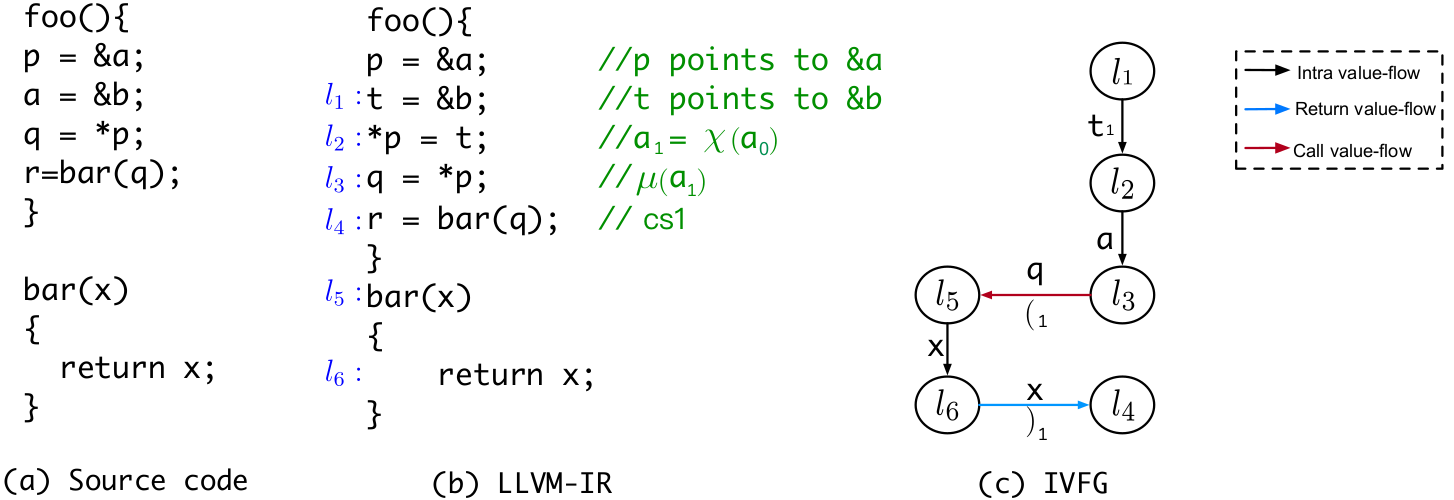
\includegraphics[width=0.6\textwidth]{figures/llvm_ir_and_ivfg.png}
            \caption{C Code fragment, its LLVM-IR and IVFG}
            \label{fig:code_fragment}
        \end{figure}
    \end{minipage}\hfill
    \begin{minipage}[m]{\linewidth}
        \begin{itemize}
            \item LLVM-IR в качестве промежуочного представления
            \item Построение IVFG на основе LLVM-IR программы
            \item $\mathcal{V} = \mathcal{O} \cup \mathcal{P}$, два типа переменных
            \item $t \xrightarrow{v} t', v \in \mathcal{V}$ def-use отношение
            \item $t \xrightarrow{p} t', p \in \mathcal{P}$ direct value-flow отношение
        \end{itemize}
    \end{minipage}
\end{frame}

\begin{frame}[fragile] \frametitle{Шаг 1: Pre-embedding (2)}
    \begin{figure}
        \centering
        \begin{subfigure}[b]{0.45\textwidth}
            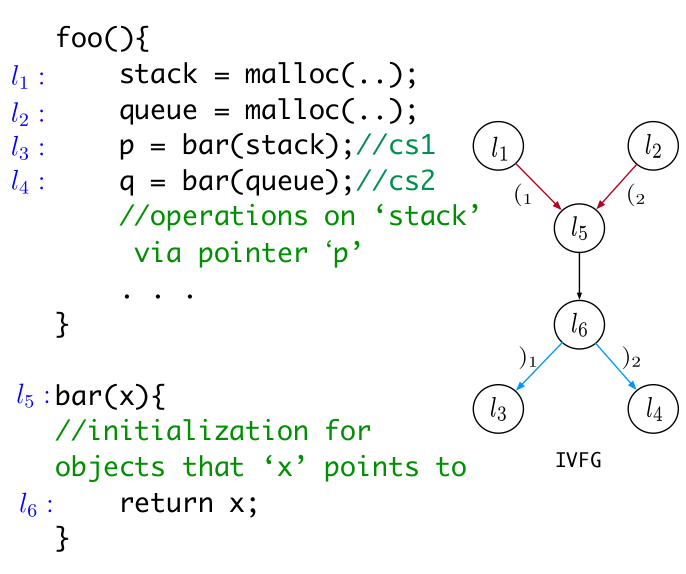
\includegraphics[width=\textwidth]{figures/pre_embeding_a.png}
            \caption{Code fragment and IVFG}
        \end{subfigure}
        \hfill
        \begin{subfigure}[b]{0.45\textwidth}
            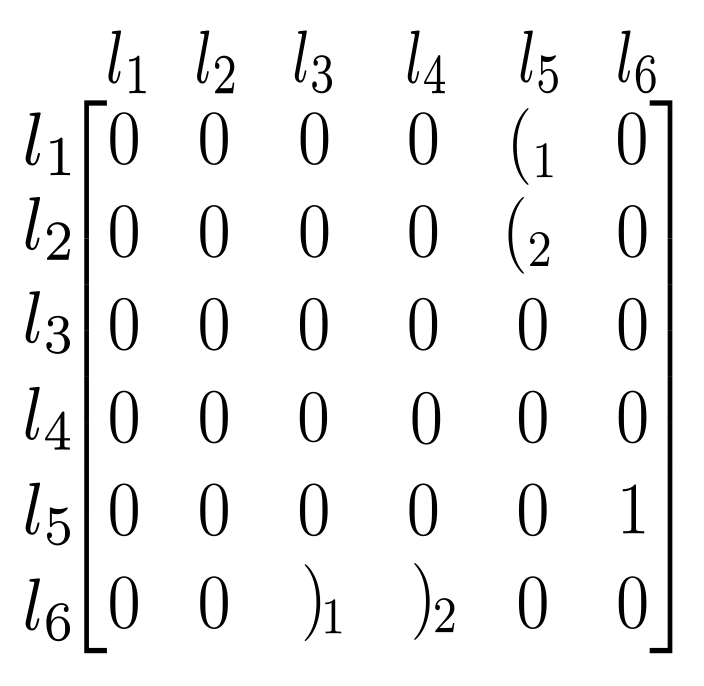
\includegraphics[width=\textwidth]{figures/pre_embedding_b.png}
            \caption{Call/return and value-flow matrix}
        \end{subfigure}
        \caption{Pre-embedding example}
    \end{figure}
\end{frame}

\begin{frame}[fragile] \frametitle{Шаг 2: Value-flow reachability via matrix multiplication}
    \begin{figure}
        \centering
        \begin{subfigure}[b]{0.2\textwidth}
            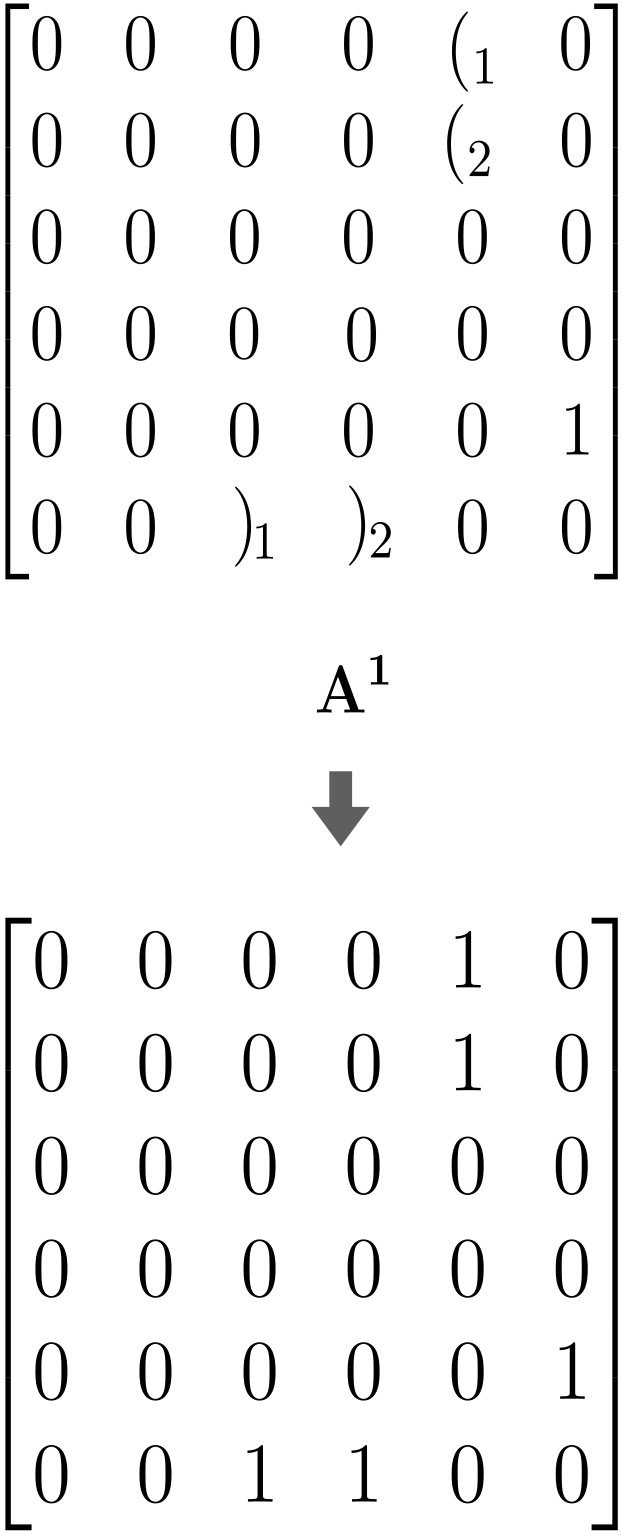
\includegraphics[width=\textwidth]{figures/cfpq_1.png}
            \caption{Matrix $A^1$}
        \end{subfigure}
        \hfill
        \begin{subfigure}[b]{0.268\textwidth}
            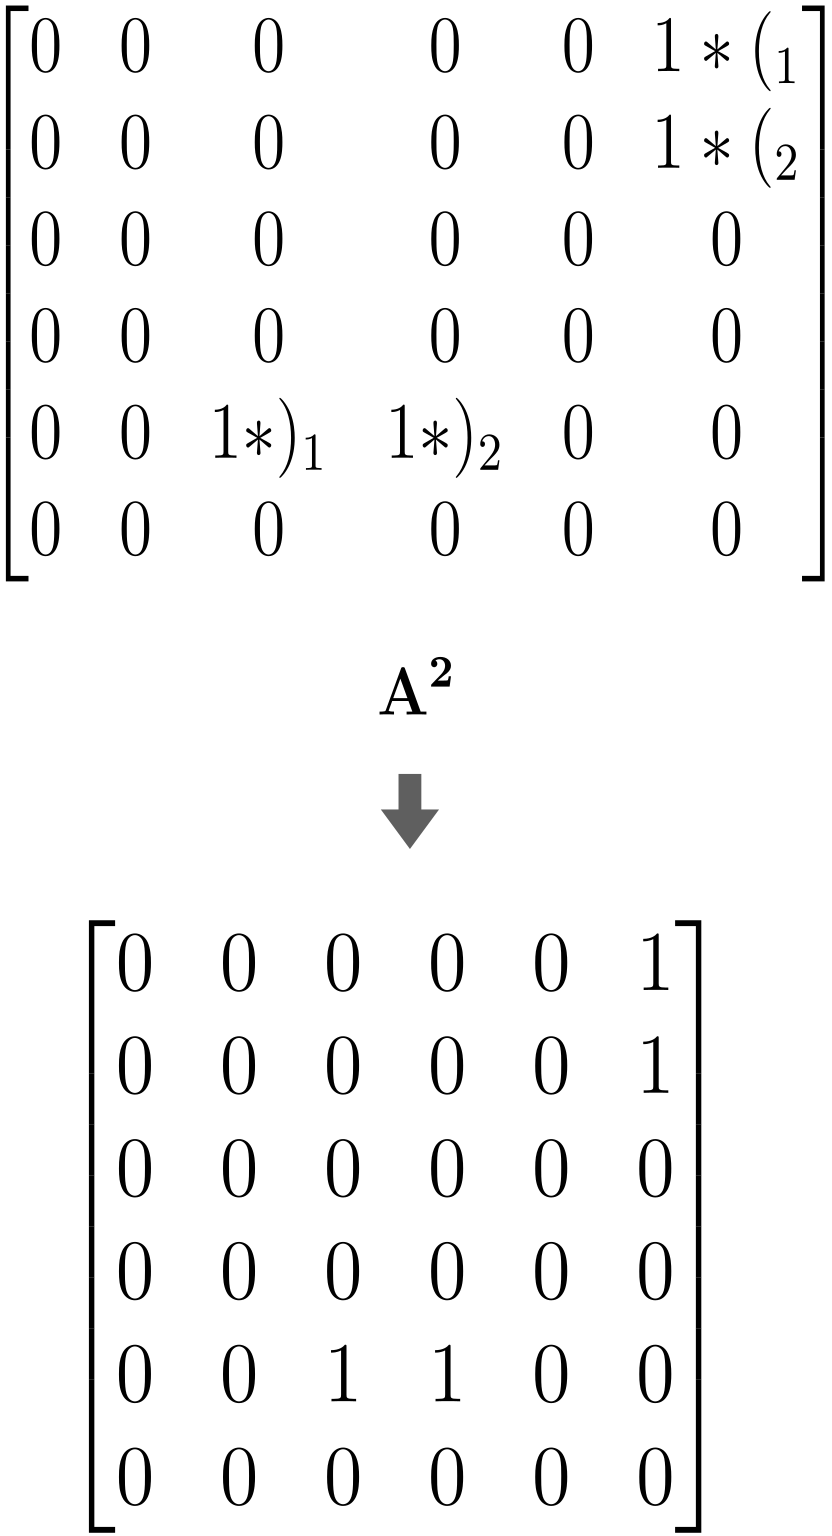
\includegraphics[width=\textwidth]{figures/cfpq_2.png}
            \caption{Matrix $A^2$}
        \end{subfigure}
        \hfill
        \begin{subfigure}[b]{0.297\textwidth}
            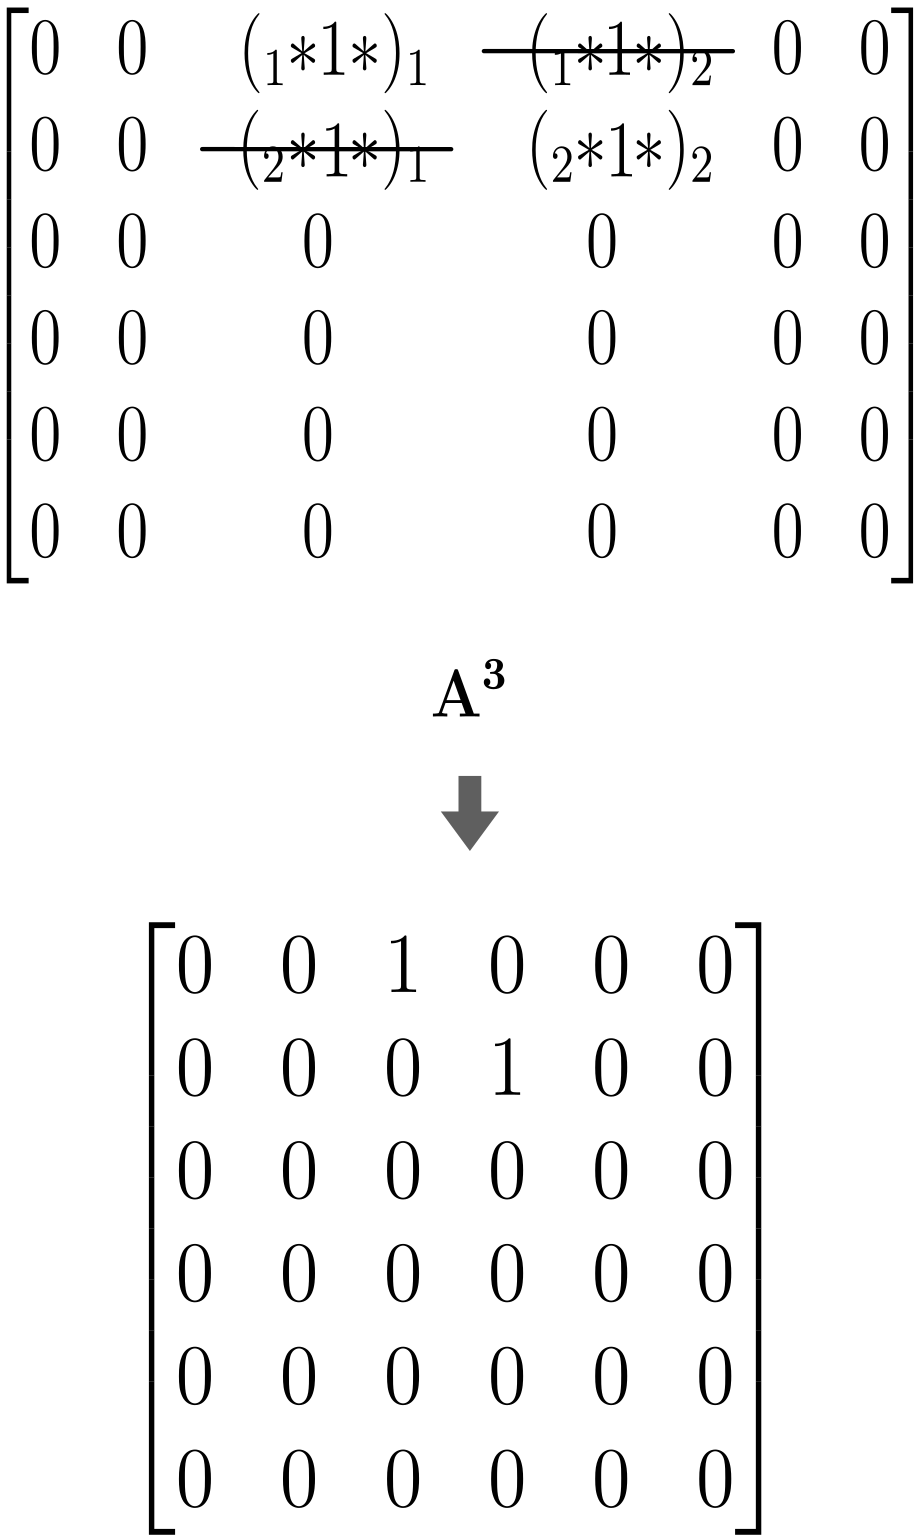
\includegraphics[width=\textwidth]{figures/cfpq_3.png}
            \caption{Matrix $A^3$}
        \end{subfigure}
        \caption{Context-sensitive value-flow reachability}
    \end{figure}
\end{frame}

\begin{frame}[fragile] \frametitle{Шаг 3: High-order proximity embedding}
    \begin{figure}
        \centering
        \begin{subfigure}[b]{0.38\textwidth}
            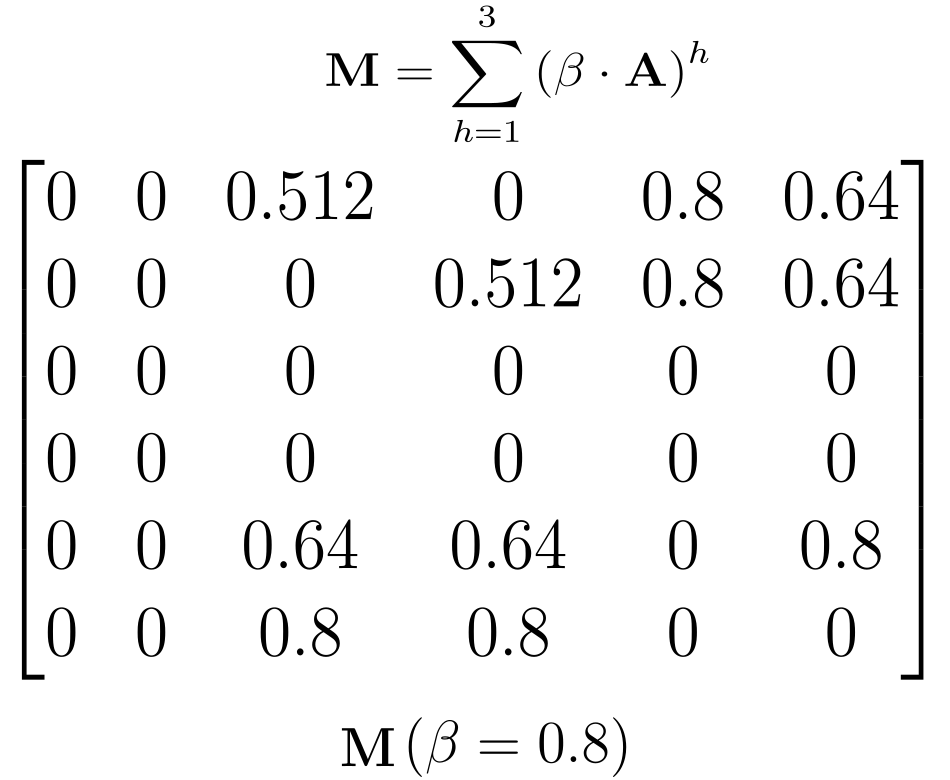
\includegraphics[width=\textwidth]{figures/proximity_matrix.png}
            \caption{High-order proximity matrix}
        \end{subfigure}
        \hfill
        \begin{subfigure}[b]{0.6\textwidth}
            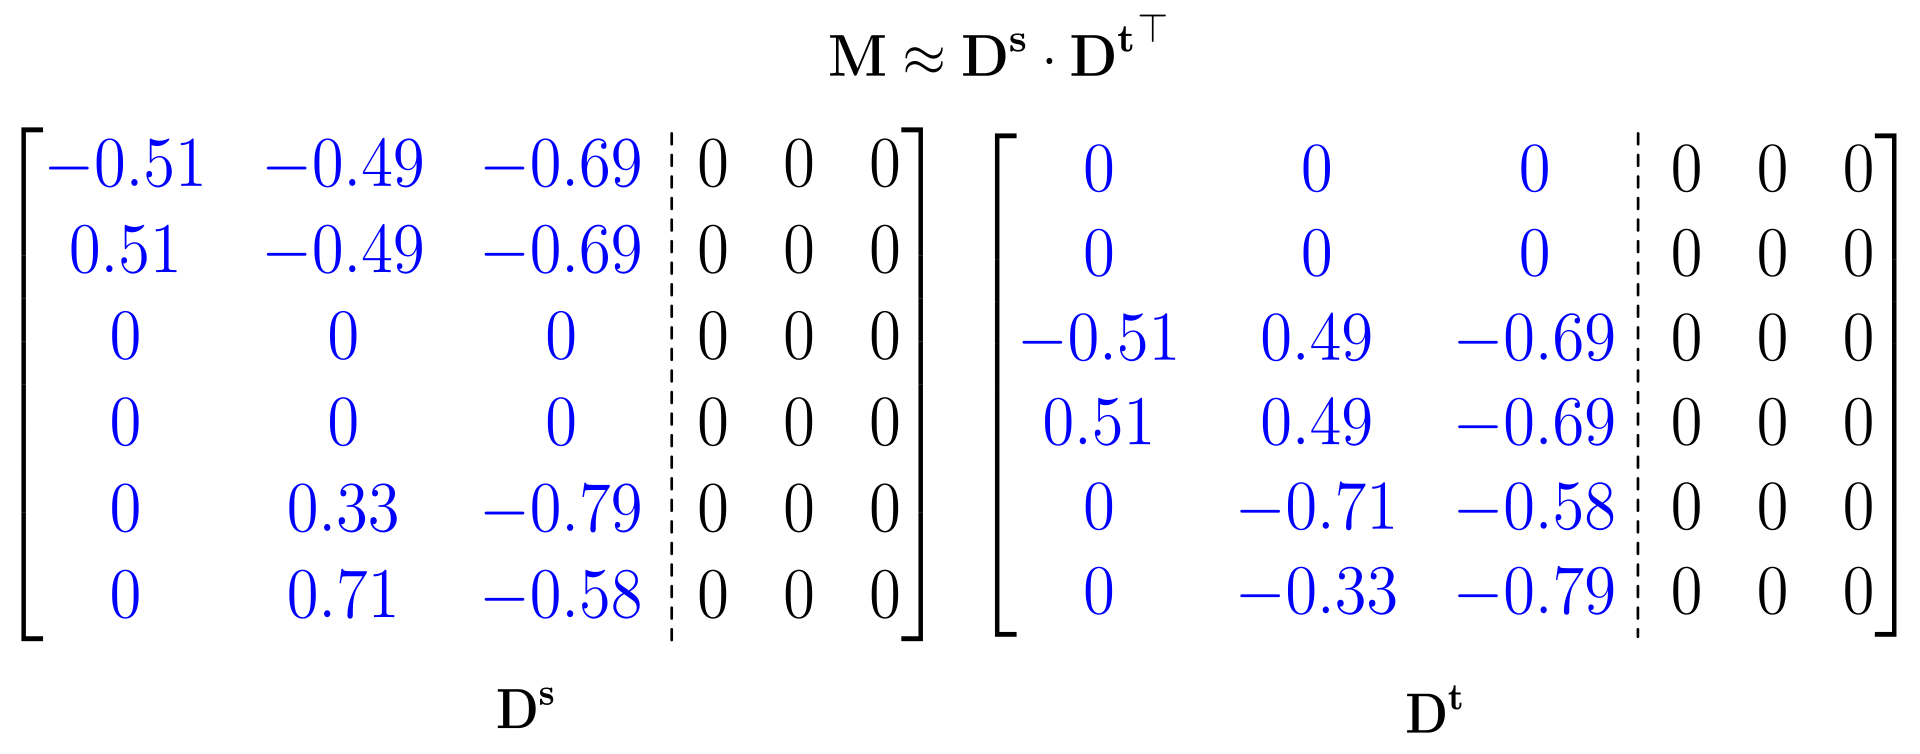
\includegraphics[width=\textwidth]{figures/embedding_vectors.png}
            \caption{Embedding vectors ($K$-factor is 3)}
        \end{subfigure}
        \caption{Embedding step}
    \end{figure}
\end{frame}

\begin{frame}[fragile] \frametitle{Шаг 4: Application scenarios}
    \begin{minipage}[m]{\linewidth}
        \begin{figure}
            \centering
            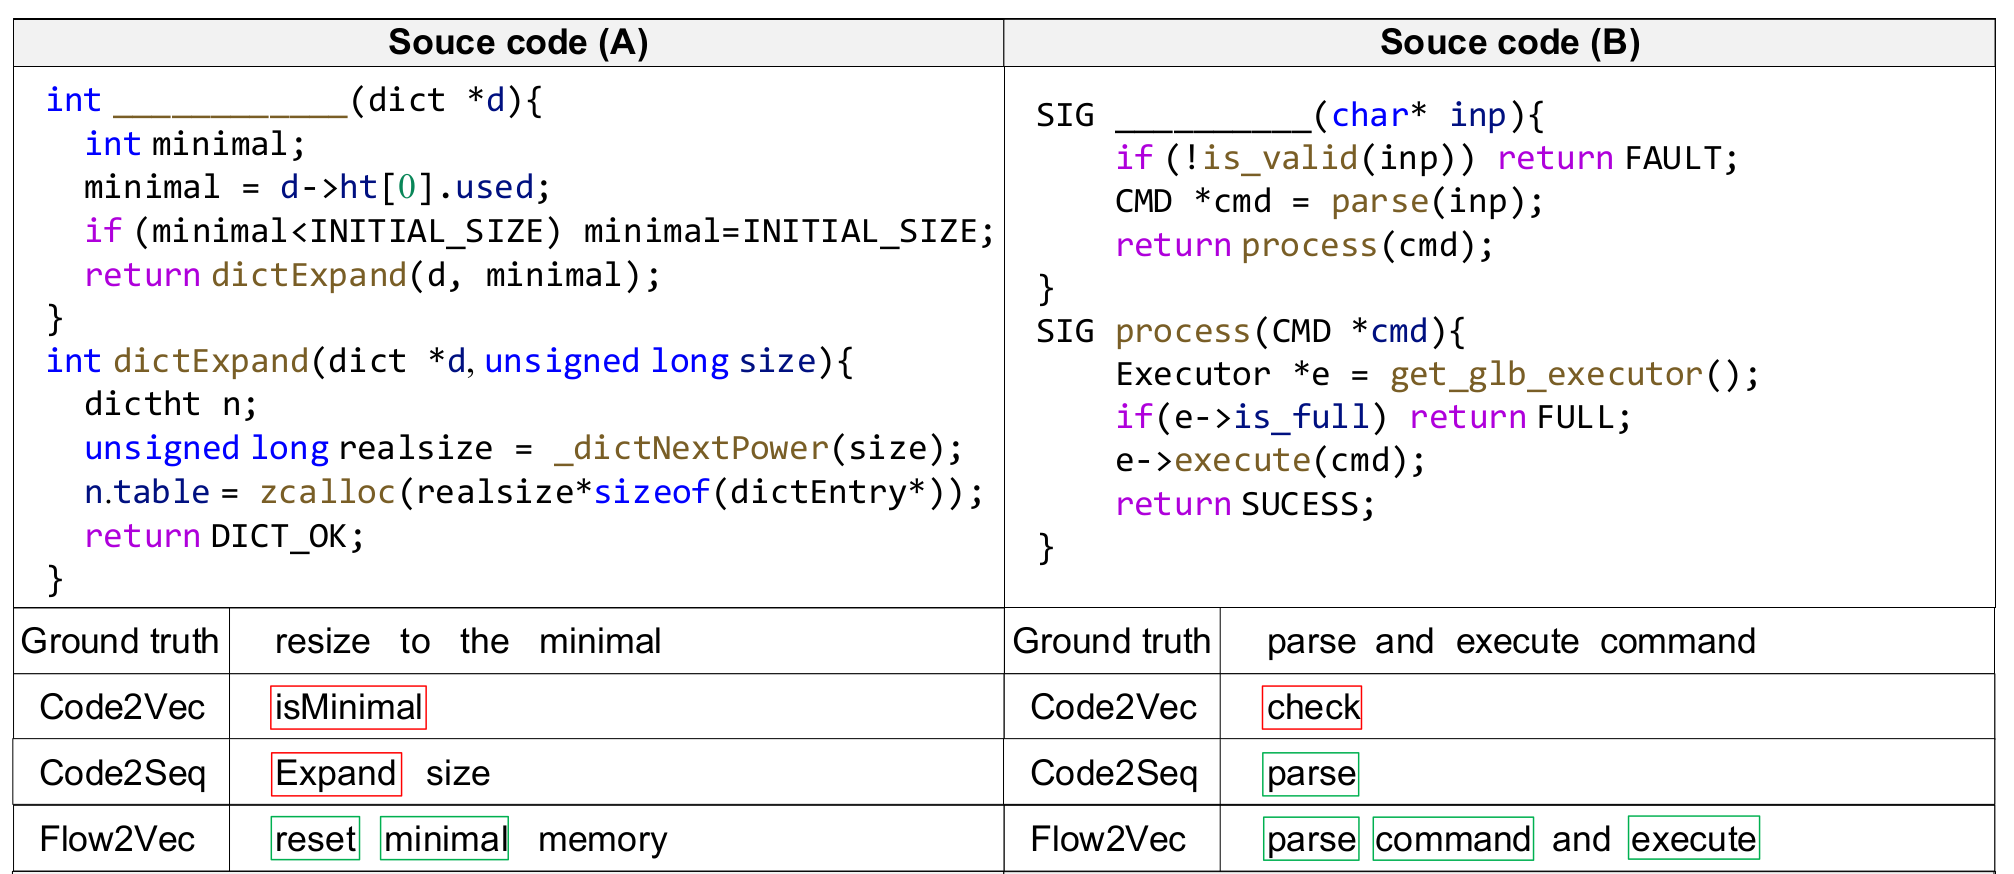
\includegraphics[width=0.7\textwidth]{figures/code_summarization_example.png}
            \caption{Code summarization example}
            \label{fig:code_summ_ex}
        \end{figure}
    \end{minipage}\hfill
    \begin{minipage}[m]{\linewidth}
        \begin{itemize}
            \item Code classification
            \item Code summarization
        \end{itemize}
    \end{minipage}
\end{frame}

\begin{frame}[fragile] \frametitle{Что мы можем предложить}
    \begin{itemize}
        \item Анализ Java программ
        \item Интсрументы для построения графов
        {
            \begin{itemize}
                \item \textbf{WALA}\footnote{ссылка: \href{https://github.com/wala/WALA}{https://github.com/wala/WALA}}
                \item \textbf{Soot}\footnote{ссылка: \href{https://github.com/soot-oss/soot}{https://github.com/soot-oss/soot}}
            \end{itemize}
        }
        \item Построение value-flow reachability матриц
        \item Построение emdebbing'а
    \end{itemize}
\end{frame}

\begin{frame}[fragile] \frametitle{CFPQ}
    \begin{itemize}
        \item Матричный Алгоритм Рустама Азимова\footnote{ссылка: \href{https://dl.acm.org/doi/10.1145/3398682.3399163}{https://dl.acm.org/doi/10.1145/3398682.3399163}}
        {
            \begin{itemize}
                \item Семантика достижимости
                \item Семантика одного пути
                \item Семантика всех путей
                \item \textit{Можем модифицировать полукольцо, чтобы считать кол-во уникальных путей}
            \end{itemize}
        }
        \item Алгоритм на основе произведения Кронекера и РА\footnote{ссылка: \href{https://link.springer.com/chapter/10.1007/978-3-030-54832-2\_6}{https://link.springer.com/chapter/10.1007/978-3-030-54832-2\_6}}
        {
            \begin{itemize}
                \item Семантика достижимости и всех путей
                \item Итеративное извлечение путей
                \item \textit{Но! На выходе нечто большее, чем просто граф}
            \end{itemize}
        }
    \end{itemize}
\end{frame}

\begin{frame}[fragile] \frametitle{Kronecker CFPQ}
    \begin{figure}
        \centering
        \begin{subfigure}[b]{0.2\textwidth}
            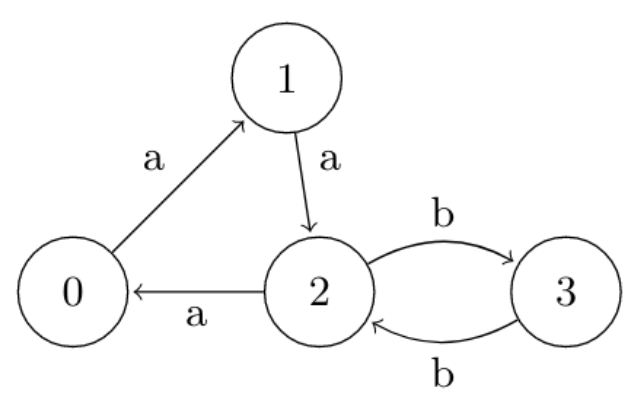
\includegraphics[width=\textwidth]{figures/graph.png}
            \caption{Input directed graph $\mathcal{G}$}
        \end{subfigure}
        \hfill
        \begin{subfigure}[b]{0.2\textwidth}
            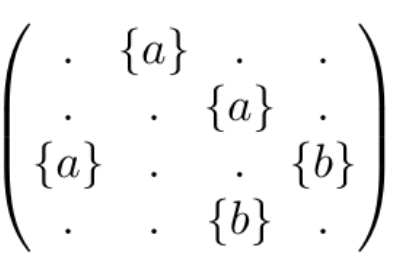
\includegraphics[width=\textwidth]{figures/graph_matrix.png}
            \caption{$\mathcal{G}$ adjacency matrix}
        \end{subfigure}
        \hfill
        \begin{subfigure}[b]{0.2\textwidth}
            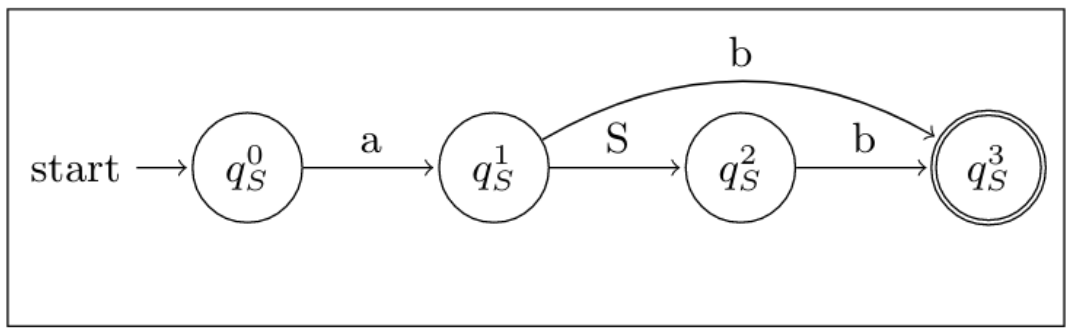
\includegraphics[width=\textwidth]{figures/automata.png}
            \caption{RSA for $S \rightarrow ab~|~aSb$}
        \end{subfigure}
        \hfill
        \begin{subfigure}[b]{0.2\textwidth}
            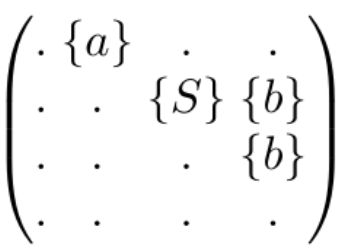
\includegraphics[width=\textwidth]{figures/automata_matrix.png}
            \caption{RSA adjacency matrix}
        \end{subfigure}
        \hfill
        \begin{subfigure}[b]{0.3\textwidth}
            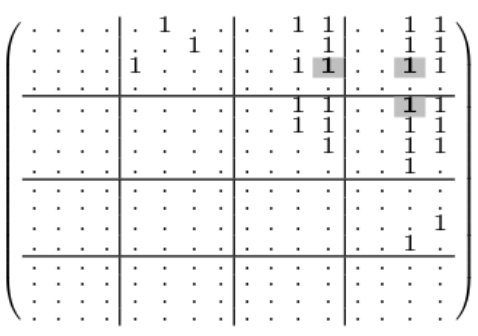
\includegraphics[width=\textwidth]{figures/kronecker_result.png}
            \caption{Result index}
        \end{subfigure}
        \caption{Kronecker CFPQ brief example}
    \end{figure}
\end{frame}

\begin{frame}[fragile] \frametitle{Заключение}
    \begin{itemize}
        \item Flow2Vec: связь анализа кода, CFPQ, и методов машинного обучения
        \item CFPQ для всех путей
        \item Вычисления на GPU
        \item Что с этим делать?
    \end{itemize}
\end{frame}

\begin{frame} \frametitle{Дополнительно}
    \begin{itemize}
        \item Почта: \href{mailto:egororachyov@gmail.com}{egororachyov@gmail.com}
        \item Материалы презентации:
        {
            \begin{itemize}
                \item Flow2Vec: Value-Flow-Based Precise Code Embedding, \\Yulei Sui, Xiao Cheng, Guanqin Zhang, Haoyu Wang, ссылка: \href{https://dl.acm.org/doi/10.1145/3428301}{https://dl.acm.org/doi/10.1145/3428301}
                \item Context-Free Path Querying with Single-Path Semantics by Matrix Multiplication, \\Arseniy Terekhov, Artyom  Khoroshev, Rustam  Azimov, Semyon Grigorev, ссылка: \href{https://dl.acm.org/doi/10.1145/3398682.3399163}{https://dl.acm.org/doi/10.1145/3398682.3399163}
                \item Context-Free Path Querying by Kronecker Product, \\Egor Orachev, Ilya Epelbaum, Rustam  Azimov, Semyon Grigorev, ссылка: \href{https://link.springer.com/chapter/10.1007/978-3-030-54832-2\_6}{https://link.springer.com/chapter/10.1007/978-3-030-54832-2\_6}
            \end{itemize}
        }
    \end{itemize}
\end{frame}

\end{document}
